% !TeX root = ../main.tex

\chapter{大模型心理健康与情绪分析系统设计与实现}

近年来,随着心理健康问题的日益严重,社会对智能化心理健康服务的需求日益增长。传统的心理健康评估和情绪分析方法通常依赖于专业心理咨询师的经验判断,而人工评估方式不仅成本高昂,且受限于个体心理咨询师的知识广度和经验深度,导致其在大规模应用中的可扩展性受限。另一方面,已有的自动化心理健康评估工具多以问卷和量表为主,缺乏对多轮对话和动态情绪变化的深入理解。在此背景下,结合大语言模型(LLM)与多模态数据处理能力的心理与情绪分析系统的研发显得尤为重要。

本文提出的大模型心理与情绪分析系统,融合了基于大模型的心理健康对话方法和语音情感描述技术,以提升心理健康评估的智能化水平。系统以大语言模型为核心,结合心理健康领域的专业数据对大模型进行微调训练,使其具备更强的心理学知识和情感理解能力。此外,除了心理健康对话支持外,该系统支持语音模态数据输入,能够通过分析语音情绪,并产生相应的情感描述,可以为心理健康从业者和用户提供辅助的情感支持服务。

本章将从下面几个方便详细介绍大模型心理与情绪分析系统的软件设计与实现过程:(1)系统分析与总体设计,需求分析根据实际的心理健康场景,设计系统的功能模块和整体架构;(2)系统功能模块设计,详细介绍系统的各个功能模块的设计和实现;(3)软件使用流程,展示系统的使用流程和操作方法。

\section{系统分析与总体设计}

\subsection{系统需求分析}

随着大语言模型(LLM)在心理健康和语音情绪分析领域的应用日益广泛,本文提出的大模型心理与情绪分析系统,旨在利用先进的自然语言处理(NLP)和多模态学习技术,为心理健康对话支持和情感分析提供有效的智能解决方案。本系统结合心理大型语言模型 PsycoLLM 和多模态情感描述生成模型 SEMO-LLM,以提升用户在心理咨询、情感对话和语音情绪分析方面的体验。

本系统旨在通过第三章实现的心理大模型 PsycoLLM 和第四章实现的多模态情感描述大模型 SEMO-LLM ,构建智能化的心理健康与情感分析平台,以提升用户的心理咨询和情感交互体验。核心目标包括智能心理问答,基于 PsycoLLM 提供高质量的心理咨询和知识问答;多轮情感交互,通过共情对话模型提升对话自然度和情境理解能力;语音情绪分析,利用SEMO-LLM对用户语音进行情感解析,并生成相应的文本提示;心理评估与反馈,基于心理咨询考试标准进行心理状态评估,提供专业反馈;用户个性化推荐,结合用户历史交互数据,优化心理咨询建议和情感描述,以实现更加精准的个性化支持。整体而言,本系统通过整合大模型的自然语言理解能力和多模态分析技术,致力于提供科学、高效、智能化的心理健康对话支持和情感分析服务。

\begin{figure}[ht]
  \centering
  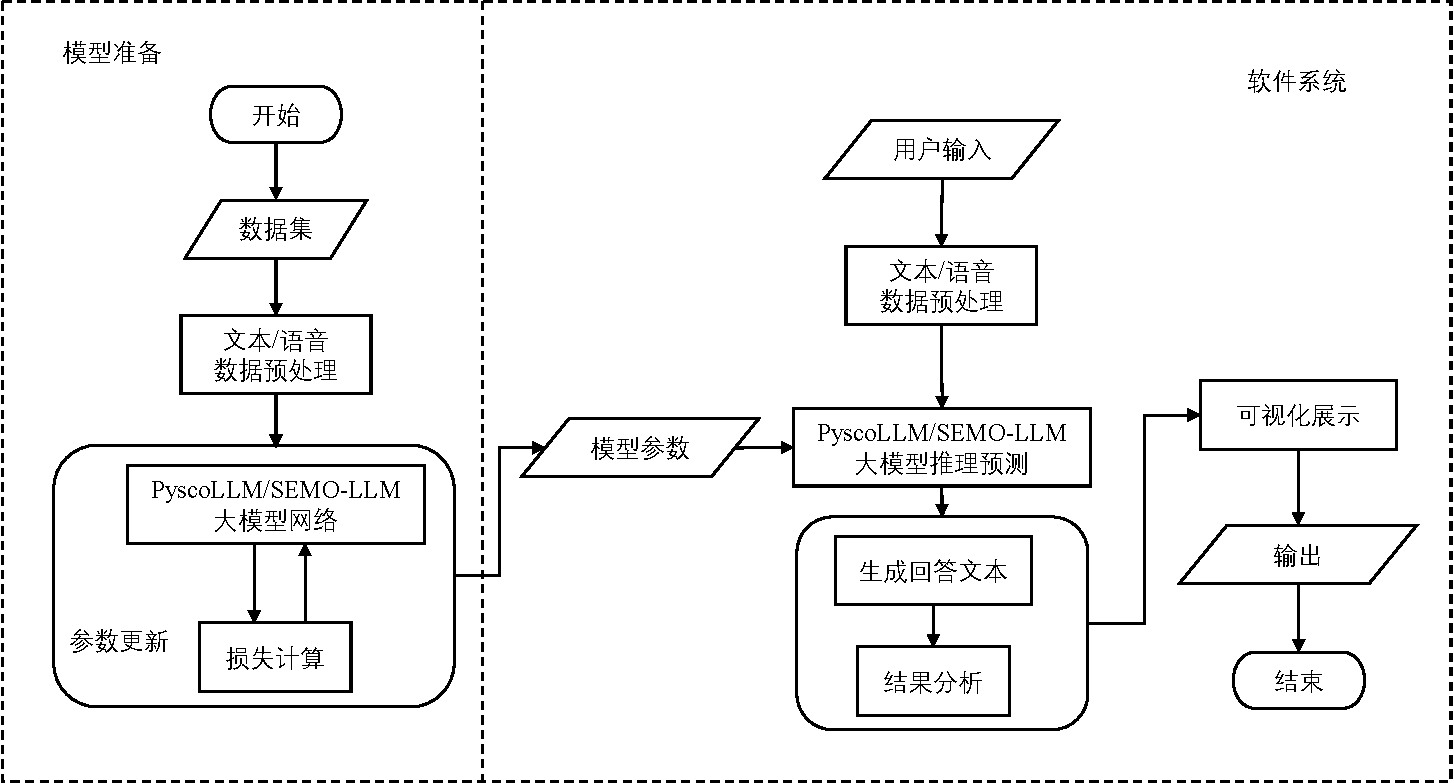
\includegraphics[width=1\textwidth]{system-design-workflow.pdf}
  \caption{系统总体流程图}
  \label{fig:system-design-workflow}
\end{figure}

本系统的功能需求可归纳为以下四个核心方面:(1)输入数据来源:系统支持文本与语音两种输入模态,用户可通过文本输入或语音输入方式进行心理咨询与情感交互,以满足不同场景下的交互需求。(2)智能心理问答:基于心理大模型 PsycoLLM,系统能够精准解析用户提出的心理健康相关问题,提供专业化的心理咨询建议与知识问答服务,同时支持多轮对话与情感交互,增强系统的互动性与共情能力。(3)语音情感描述:系统采用SEMO-LLM 进行语音情感分析,能够从用户语音输入中提取情绪特征,如语调、音强、语速等,并基于此生成相应的文本描述,以帮助用户理解自身情绪状态,实现更深入的情感交互。(4)可视化展示:系统支持将心理咨询与情感分析的结果以可视化方式呈现,包括文本流式输出、情感趋势图、心理评估报告等,使用户能够更加直观、清晰地理解分析结果。此外,系统界面设计遵循用户体验优化原则,确保操作流程流畅,界面布局简洁美观,以提升用户的交互体验和使用便捷性。

\subsection{系统总体设计}

本系统采用第三章所训练的心理大模型 PsycoLLM 与第四章所训练的多模态情感描述大模型 SEMO-LLM 模型,结合文本与语音数据,为心理健康咨询和情感分析提供智能化服务。系统主要由模型准备和软件系统两部分组成。在模型准备阶段,系统收集网络数据和用户输入的文本及语音信息,并通过数据预处理模块进行清洗、特征提取及格式转换。随后,处理后的数据被用于训练 PsycoLLM 和 SEMO-LLM 模型,并通过损失计算进行参数优化,以提高模型的心理问答和情感分析能力。

在软件系统部分,用户输入的文本或语音数据经过相应的预处理后,被送入训练好的 PsycoLLM/SEMO-LLM 模型进行推理预测,生成相应的心理咨询建议或情感描述。系统对模型输出的文本进行结果分析,预测结果通过可视化模块呈现给用户。通过不断优化数据处理和模型训练,提高系统在心理健康和情感分析场景中的实用性和准确性。系统总体流程如图~\ref{fig:system-design-workflow}所示。

\section{系统功能模块设计}

\subsection{开发环境}

大模型心理与情绪分析系统所涉及的心理大模型 PsycoLLM 和多模态情感描述大模型 SEMO-LLM 训练并部署在 Ubuntu 22.04.4 LTS 平台上,处理器为 Intel(R) Xeon(R) Gold 6326 CPU @ 2.90GHz,GPU 为 8 卡 NVIDIA A800 80G Tensor Core GPU。系统的软件开发环境使用 Visual Studio Code,Python 版本为 3.11.9,PyTorch 版本为 2.4.0,CUDA 版本为 12.4。系统的展示交互界面设计使用 Graio 4.44.1 完成,Gradio 允许开发者快速创建交互式演示,使用户可以直接在浏览器中与模型交互,而无需编写复杂的前端代码。

\subsection{系统功能}

根据系统的功能需求,本文的大模型心理与情绪分析系统设计了四个核心功能模块,分别为数据输入模块、智能心理问答模块、语音情感描述模块和可视化展示模块。这些模块协同工作,为用户提供高效、精准的心理健康咨询和情感分析服务。系统功能设计如图 ~\ref{fig:system-function-modules} 所示。

\begin{figure}[ht]
  \centering
  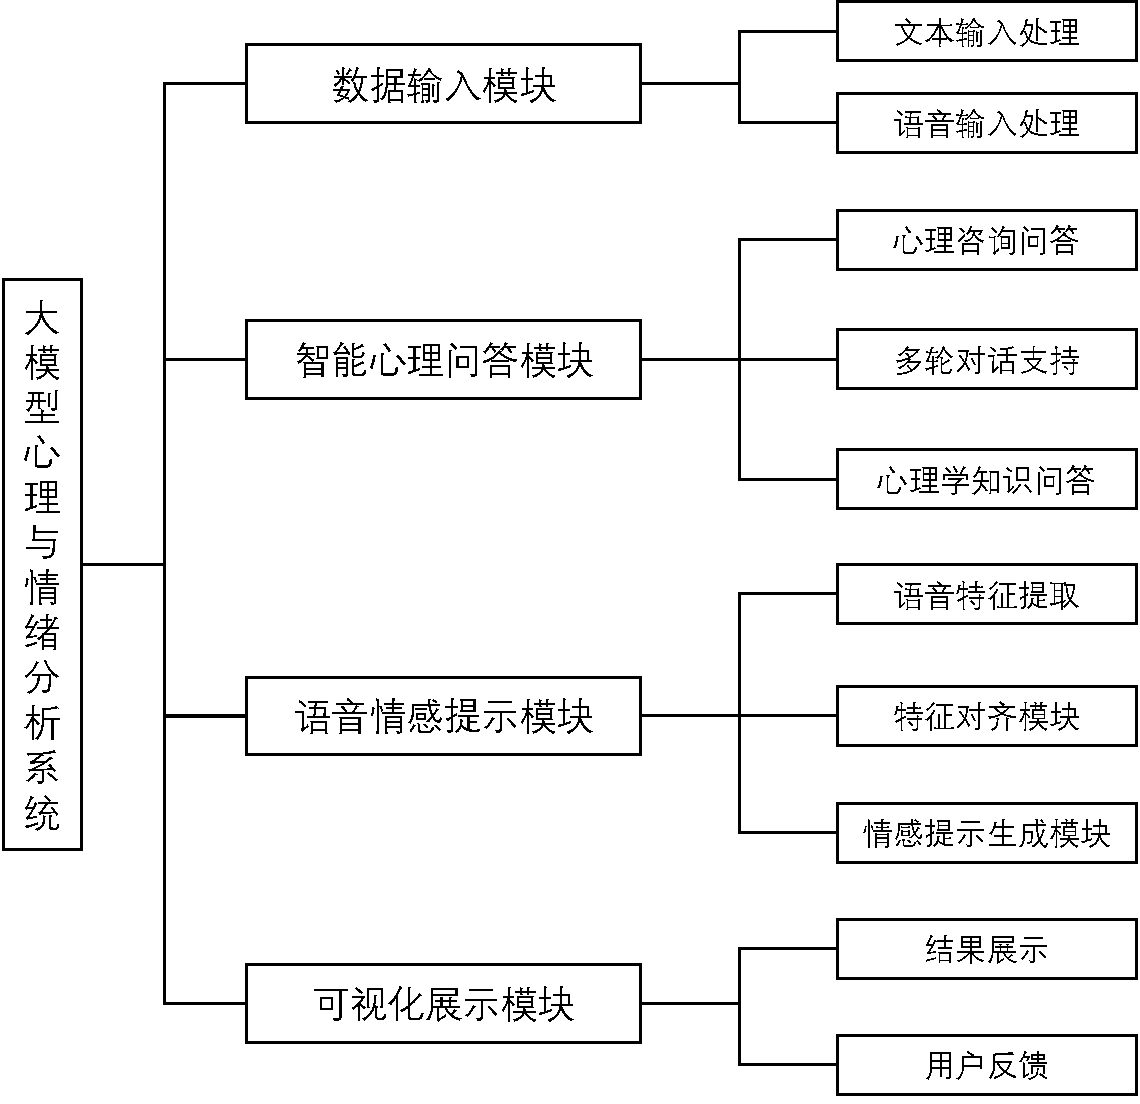
\includegraphics[width=1\textwidth]{system-function-modules.pdf}
  \caption{系统功能设计图}
  \label{fig:system-function-modules}
\end{figure}

\textbf{1. 数据输入模块}

数据输入模块的主要职责是接收用户提供的文本或语音数据,并对其进行预处理,以确保数据的质量和可用性。该模块包括两个核心功能:(1)文本输入处理。系统对输入文本执行格式标准化,如去除多余空格和换行符等,同时采用敏感词检测算法(基于 BERT 的文本分类)对内容进行审查,筛除违规或敏感词汇,以保证系统输出的安全性与合规性。(2)语音输入处理。该模块支持用户通过麦克风实时录制语音或上传语音文件(支持 MP3、WAV 等格式)。利用 WavLM-Large 模型提取语音特征,包括情感信息、音调、音强和语速等,并通过自动语音识别(ASR)技术将语音转换为文本,以便进一步进行心理问答或情感分析。

\textbf{2. 智能心理问答模块}

智能心理问答模块基于第三章构建的心理大模型 PsycoLLM,旨在提供心理健康领域的智能问答与情感对话支持。该模块的核心功能包括:(1)心理咨询问答:用户可输入心理健康相关问题,系统基于 PsycoLLM 训练过程中学习到的心理学知识,生成科学、合理的咨询建议,以辅助心理健康支持。(2)多轮对话支持:PsycoLLM 在训练过程中融入多轮对话数据进行微调,使其能够在用户交互过程中保留上下文信息,从而提供更加自然、连贯的心理对话体验。(3)心理学知识问答:用户可咨询心理学相关理论知识,如认知行为疗法(CBT)、人本主义心理学等。系统结合心理学教材与专业数据库,提供准确、权威的理论解答,以满足用户的专业学习与科普需求。

\textbf{3. 语音情感描述模块}

语音情感描述模块基于第四章构建的多模态情感描述大模型 SEMO-LLM,通过语音数据分析用户的情绪状态,并生成相应的情感描述信息。该模块的主要功能包括:(1)语音特征提取:采用 WavLM-Large 模型提取语音特征,包括音调、音强、语速及情绪状态等,为后续情感分析提供基础数据。(2)特征对齐模块:利用稀疏桥接 Transformer 模块,将提取的语音特征映射到文本特征空间,并与 Prompt 提示词 “请用一句话描述给定音频中说话人所表达的情绪” 的文本特征进行拼接对齐,确保跨模态数据的一致性。(3)情感描述生成:采用自回归解码方法,在 SEMO-LLM 中生成相应的情感描述文本,从而实现对用户情绪状态的自然语言表述。

\textbf{4. 可视化展示模块}

可视化展示模块 负责对系统的分析结果进行直观呈现,以提升用户体验和交互效果。该模块的主要功能包括:(1)结果展示:对 智能心理问答模块 和 语音情感描述模块 的输出内容进行可视化呈现。采用流式解码方式,实现心理咨询建议、情感描述文本等内容的实时动态展示,提升信息获取的直观性与即时性。(2)用户反馈:提供用户交互接口,使用户能够对系统生成的咨询建议进行评分与反馈,从而优化模型性能并提升系统的智能化水平。

此外,系统可视化界面示例如下所示:(1)心理咨询结果展示,如图 \ref{fig:心理咨询结果展示} 所示;(2)多轮对话支持展示,如图 \ref{fig:多轮对话支持展示} 所示;(3)心理学知识问答展示,如图 \ref{fig:心理知识问答展示} 所示;(4)心理健康诊断结果展示,如图 \ref{fig:心理健康诊断结果展示} 所示;(5)语音情感描述结果展示,如图 \ref{fig:语音情感描述结果展示} 所示。

\begin{figure}[ht]
  \centering
  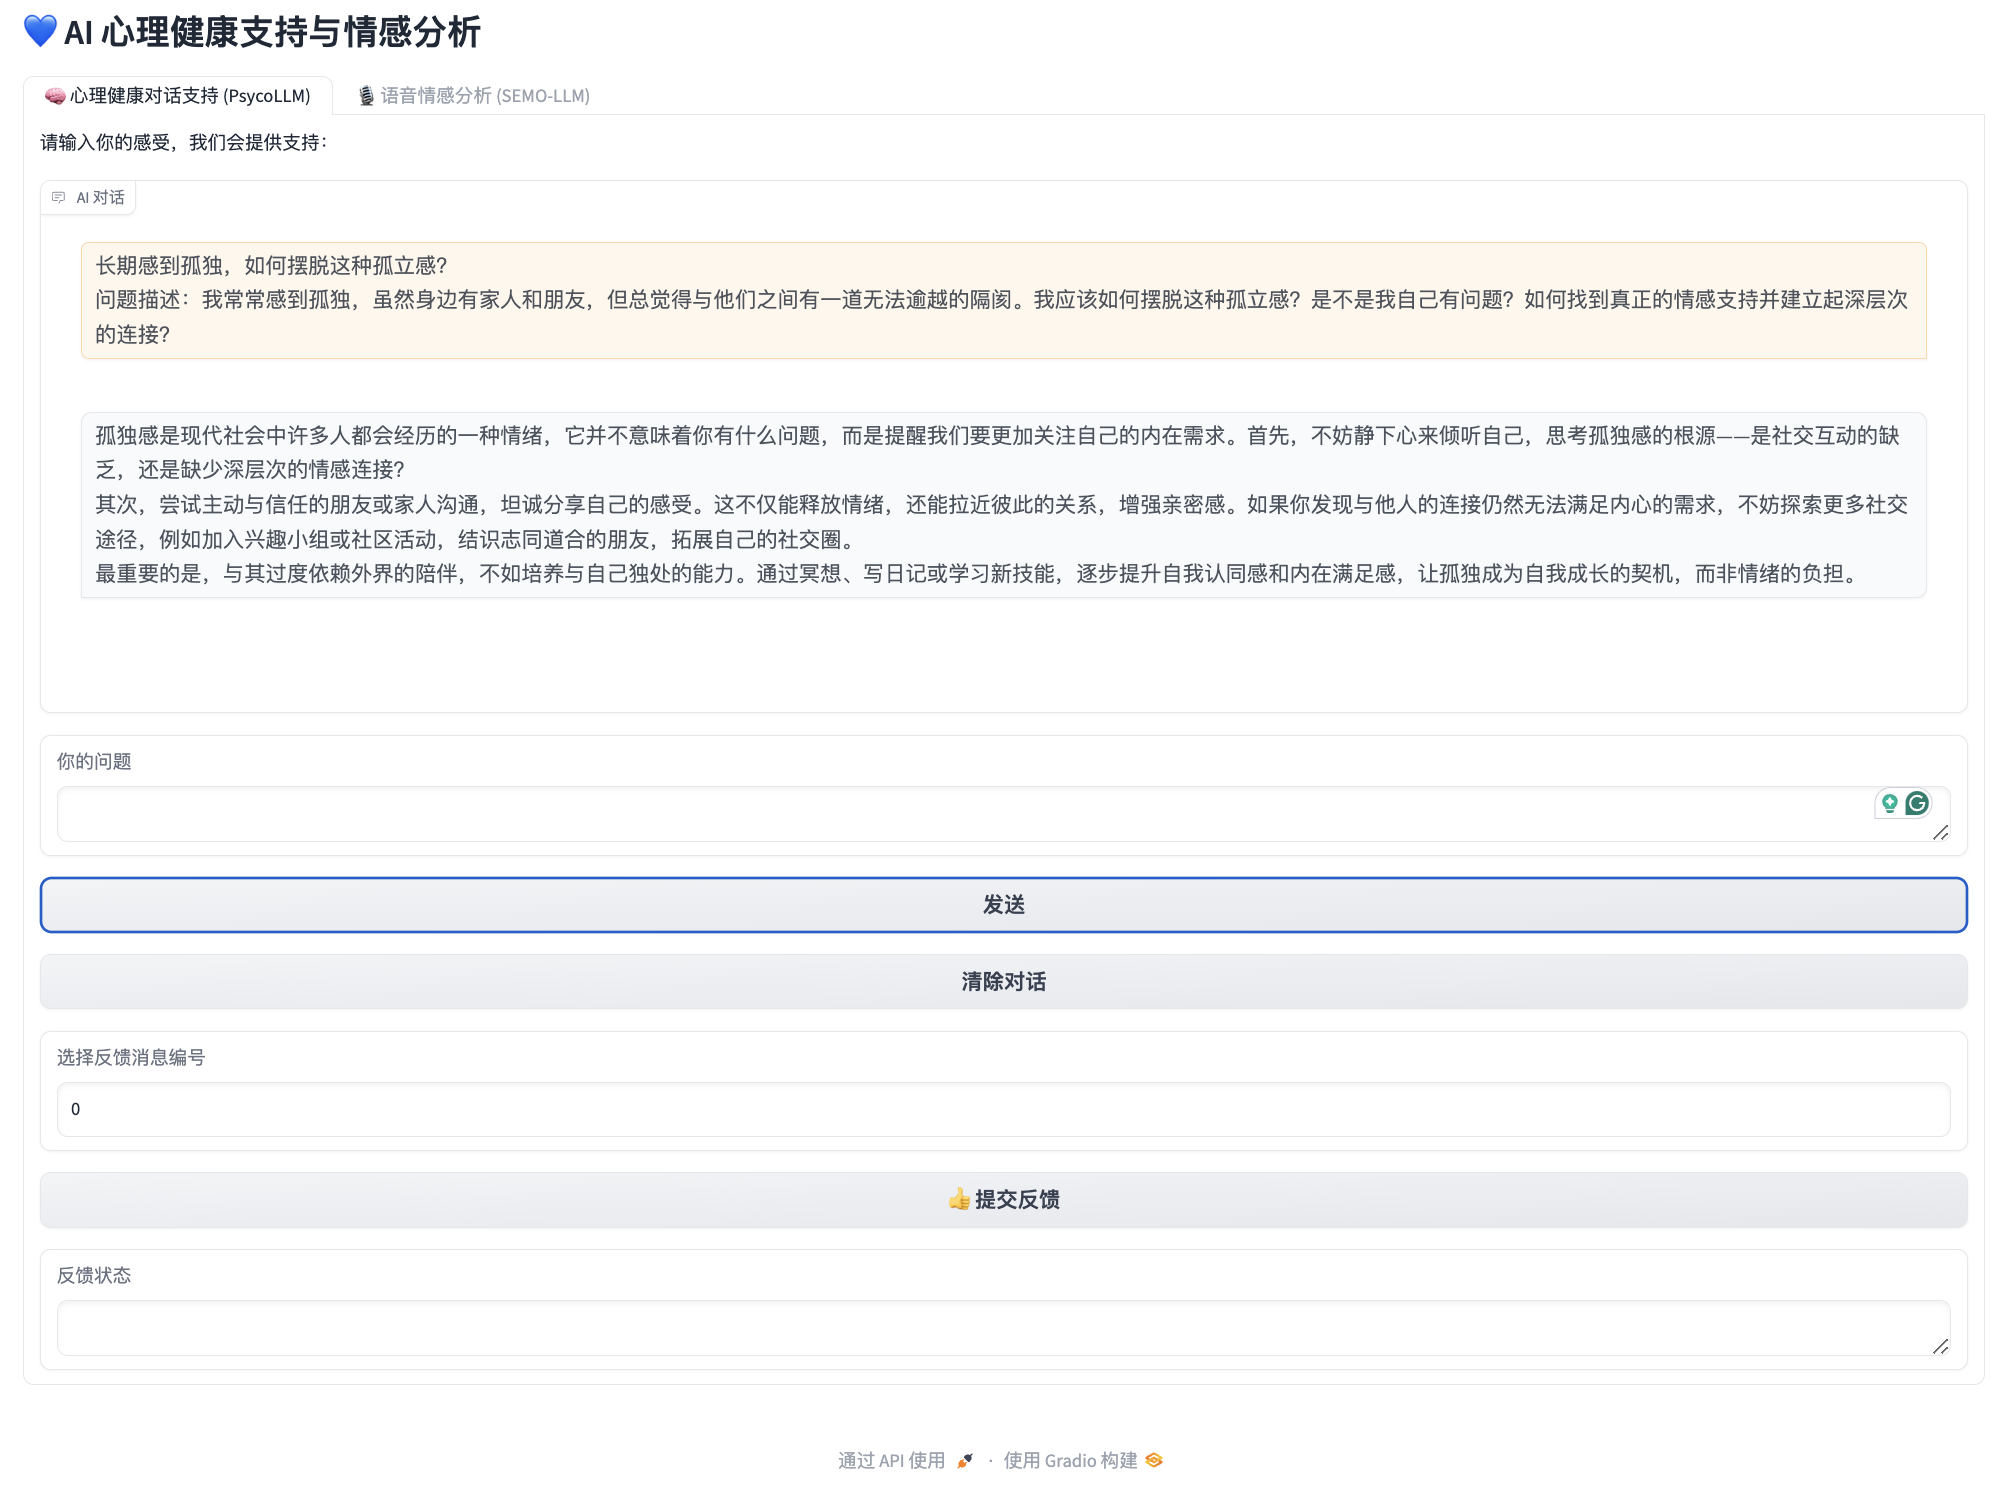
\includegraphics[width=1\textwidth]{demo1.png}
  \caption{心理咨询结果展示}
  \label{fig:心理咨询结果展示}
\end{figure}

\begin{figure}[ht]
  \centering
  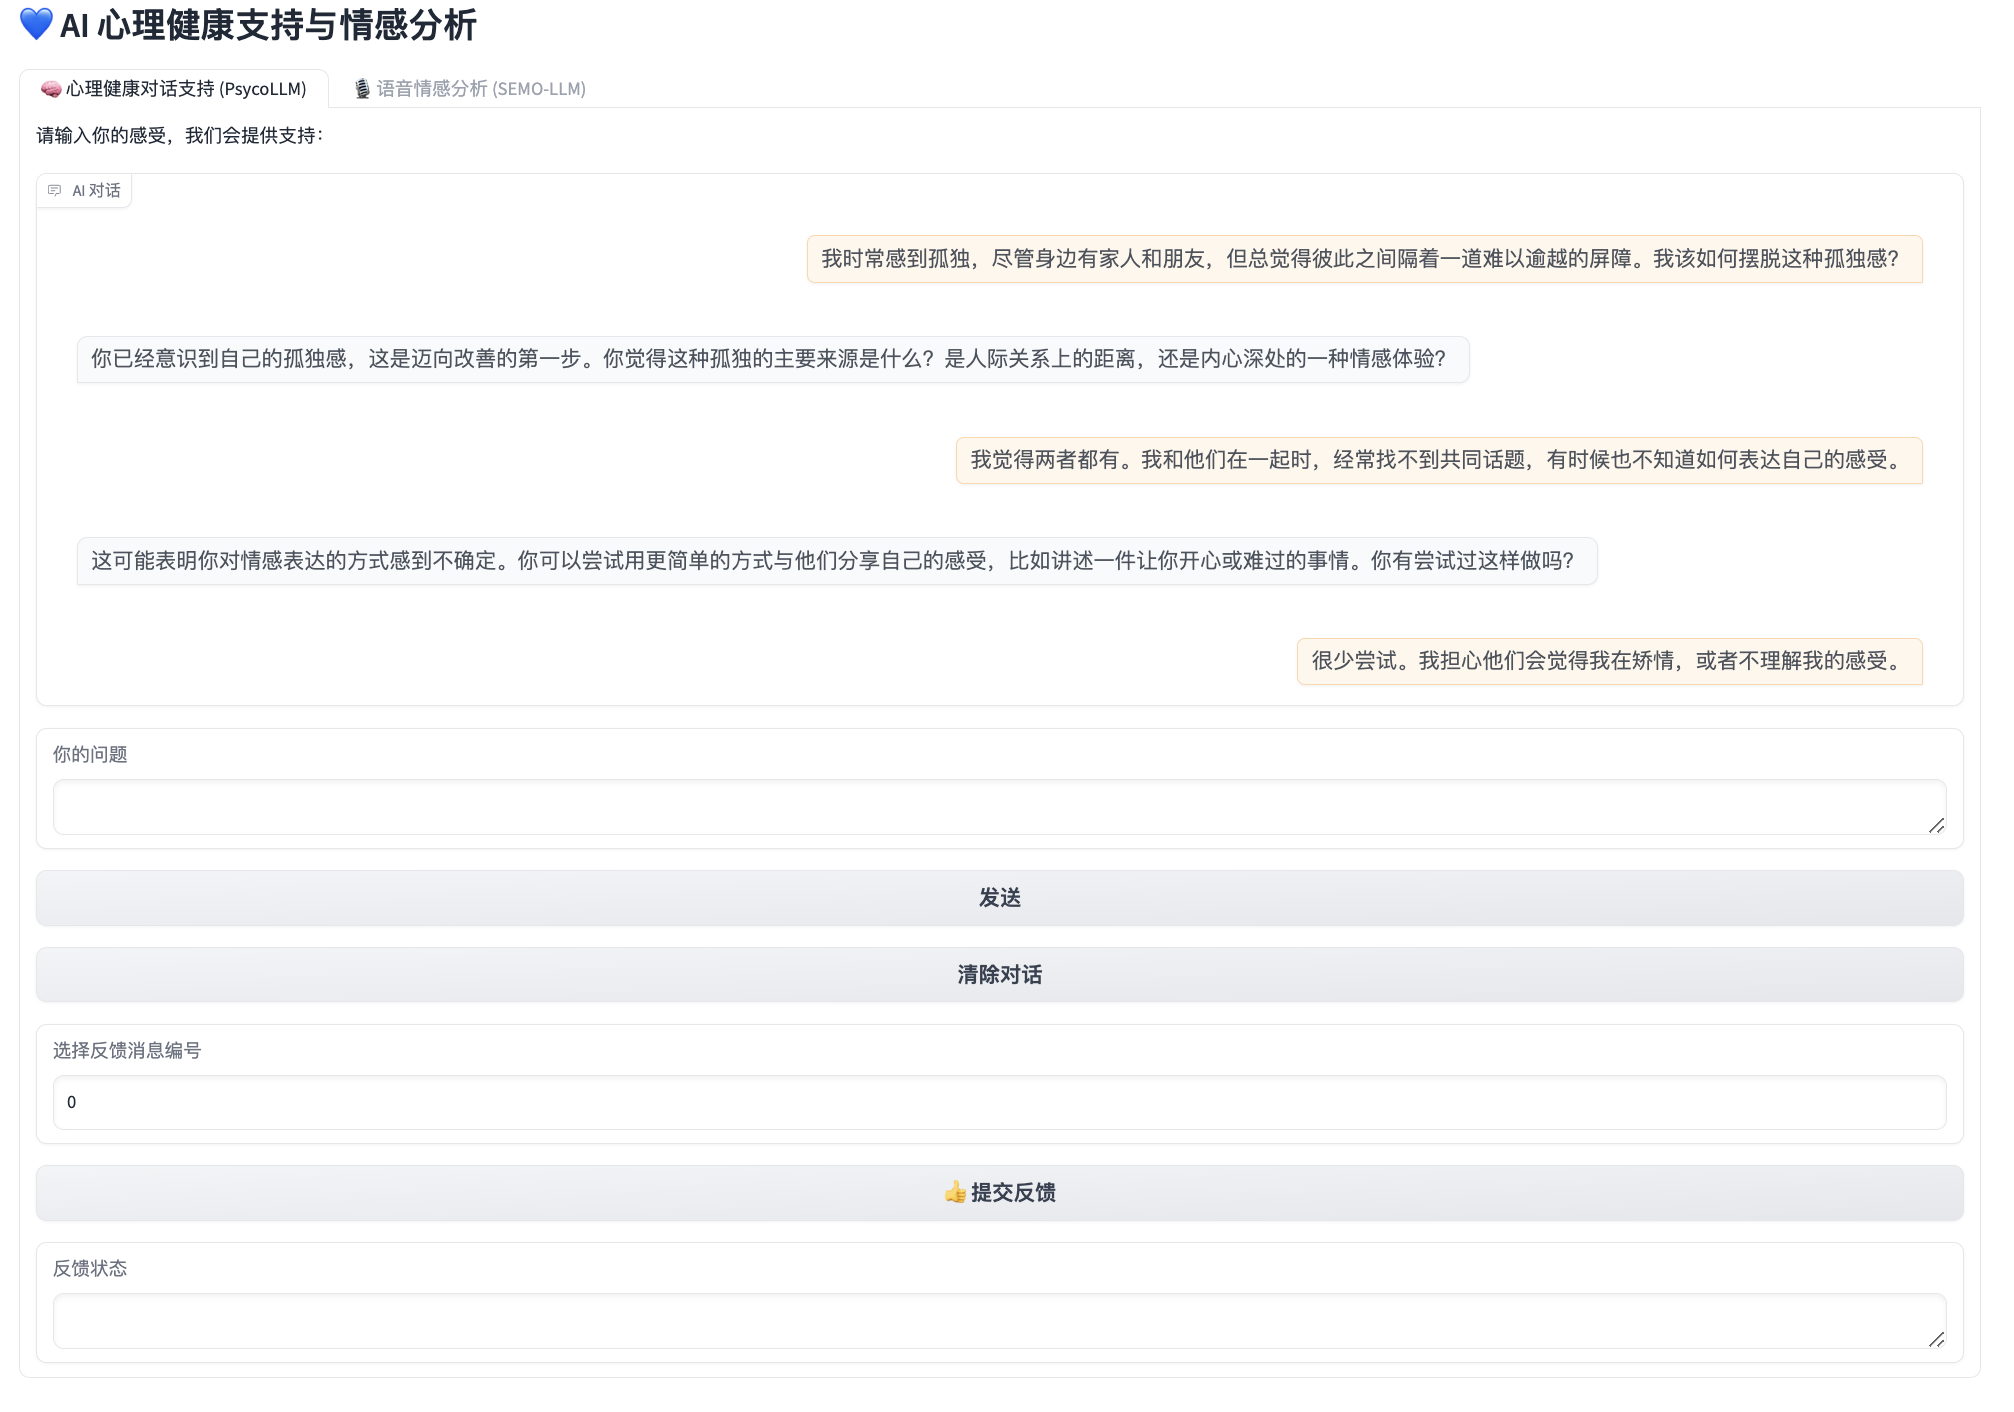
\includegraphics[width=1\textwidth]{demo2.png}
  \caption{多轮对话支持展示}
  \label{fig:多轮对话支持展示}
\end{figure}

\begin{figure}[ht]
  \centering
  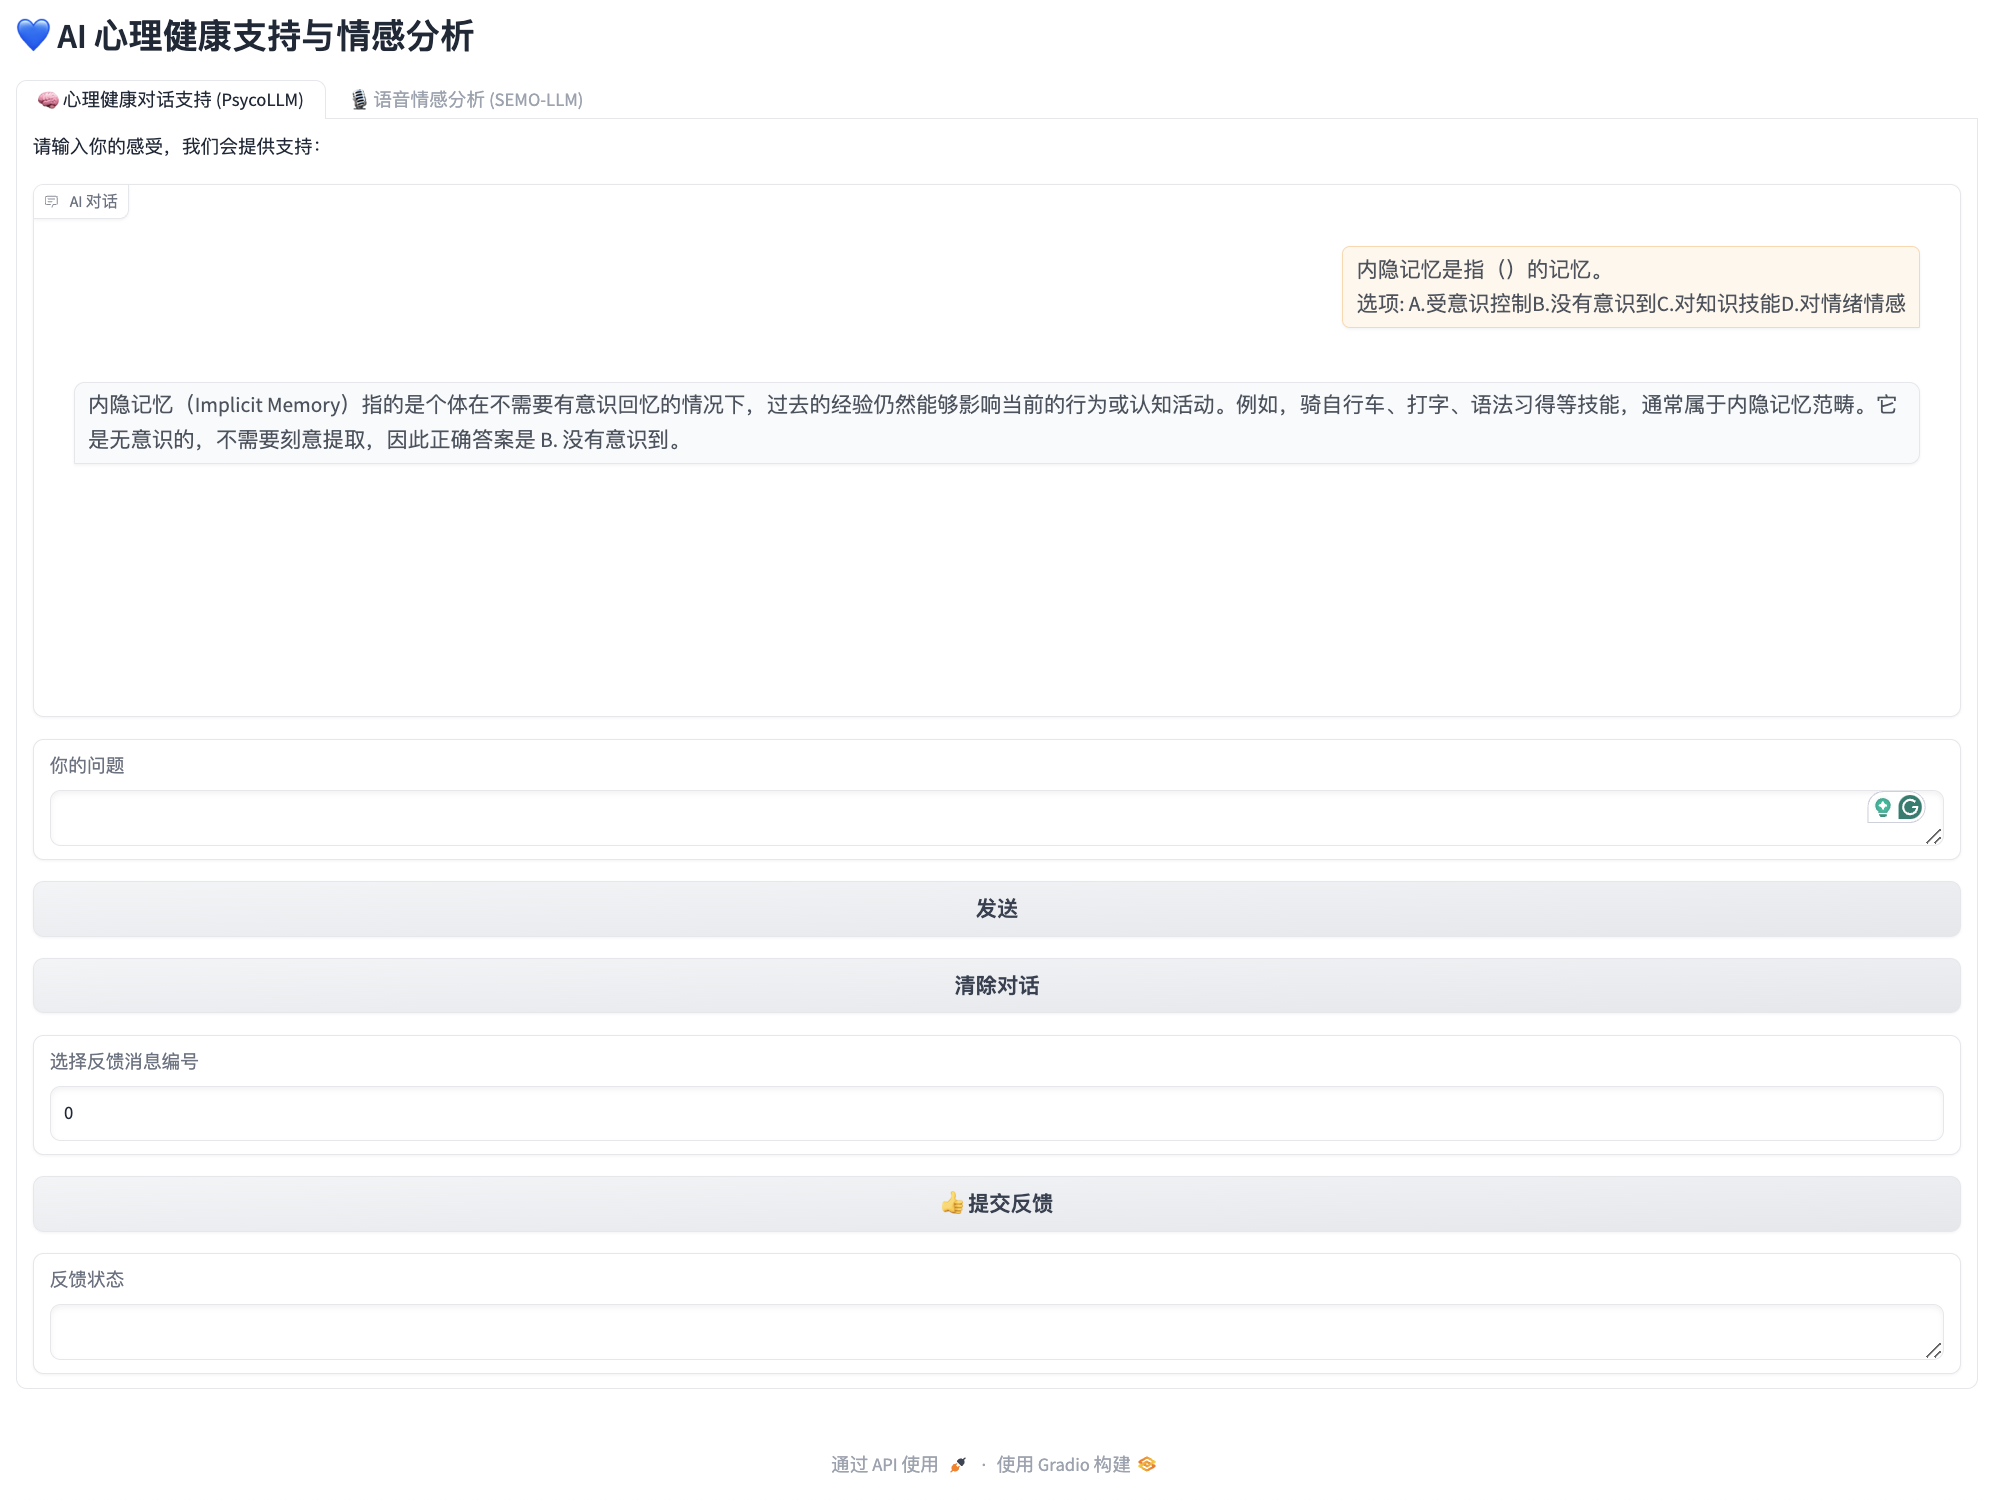
\includegraphics[width=1\textwidth]{demo3.png}
  \caption{心理知识问答展示}
  \label{fig:心理知识问答展示}
\end{figure}

\begin{figure}[ht]
  \centering
  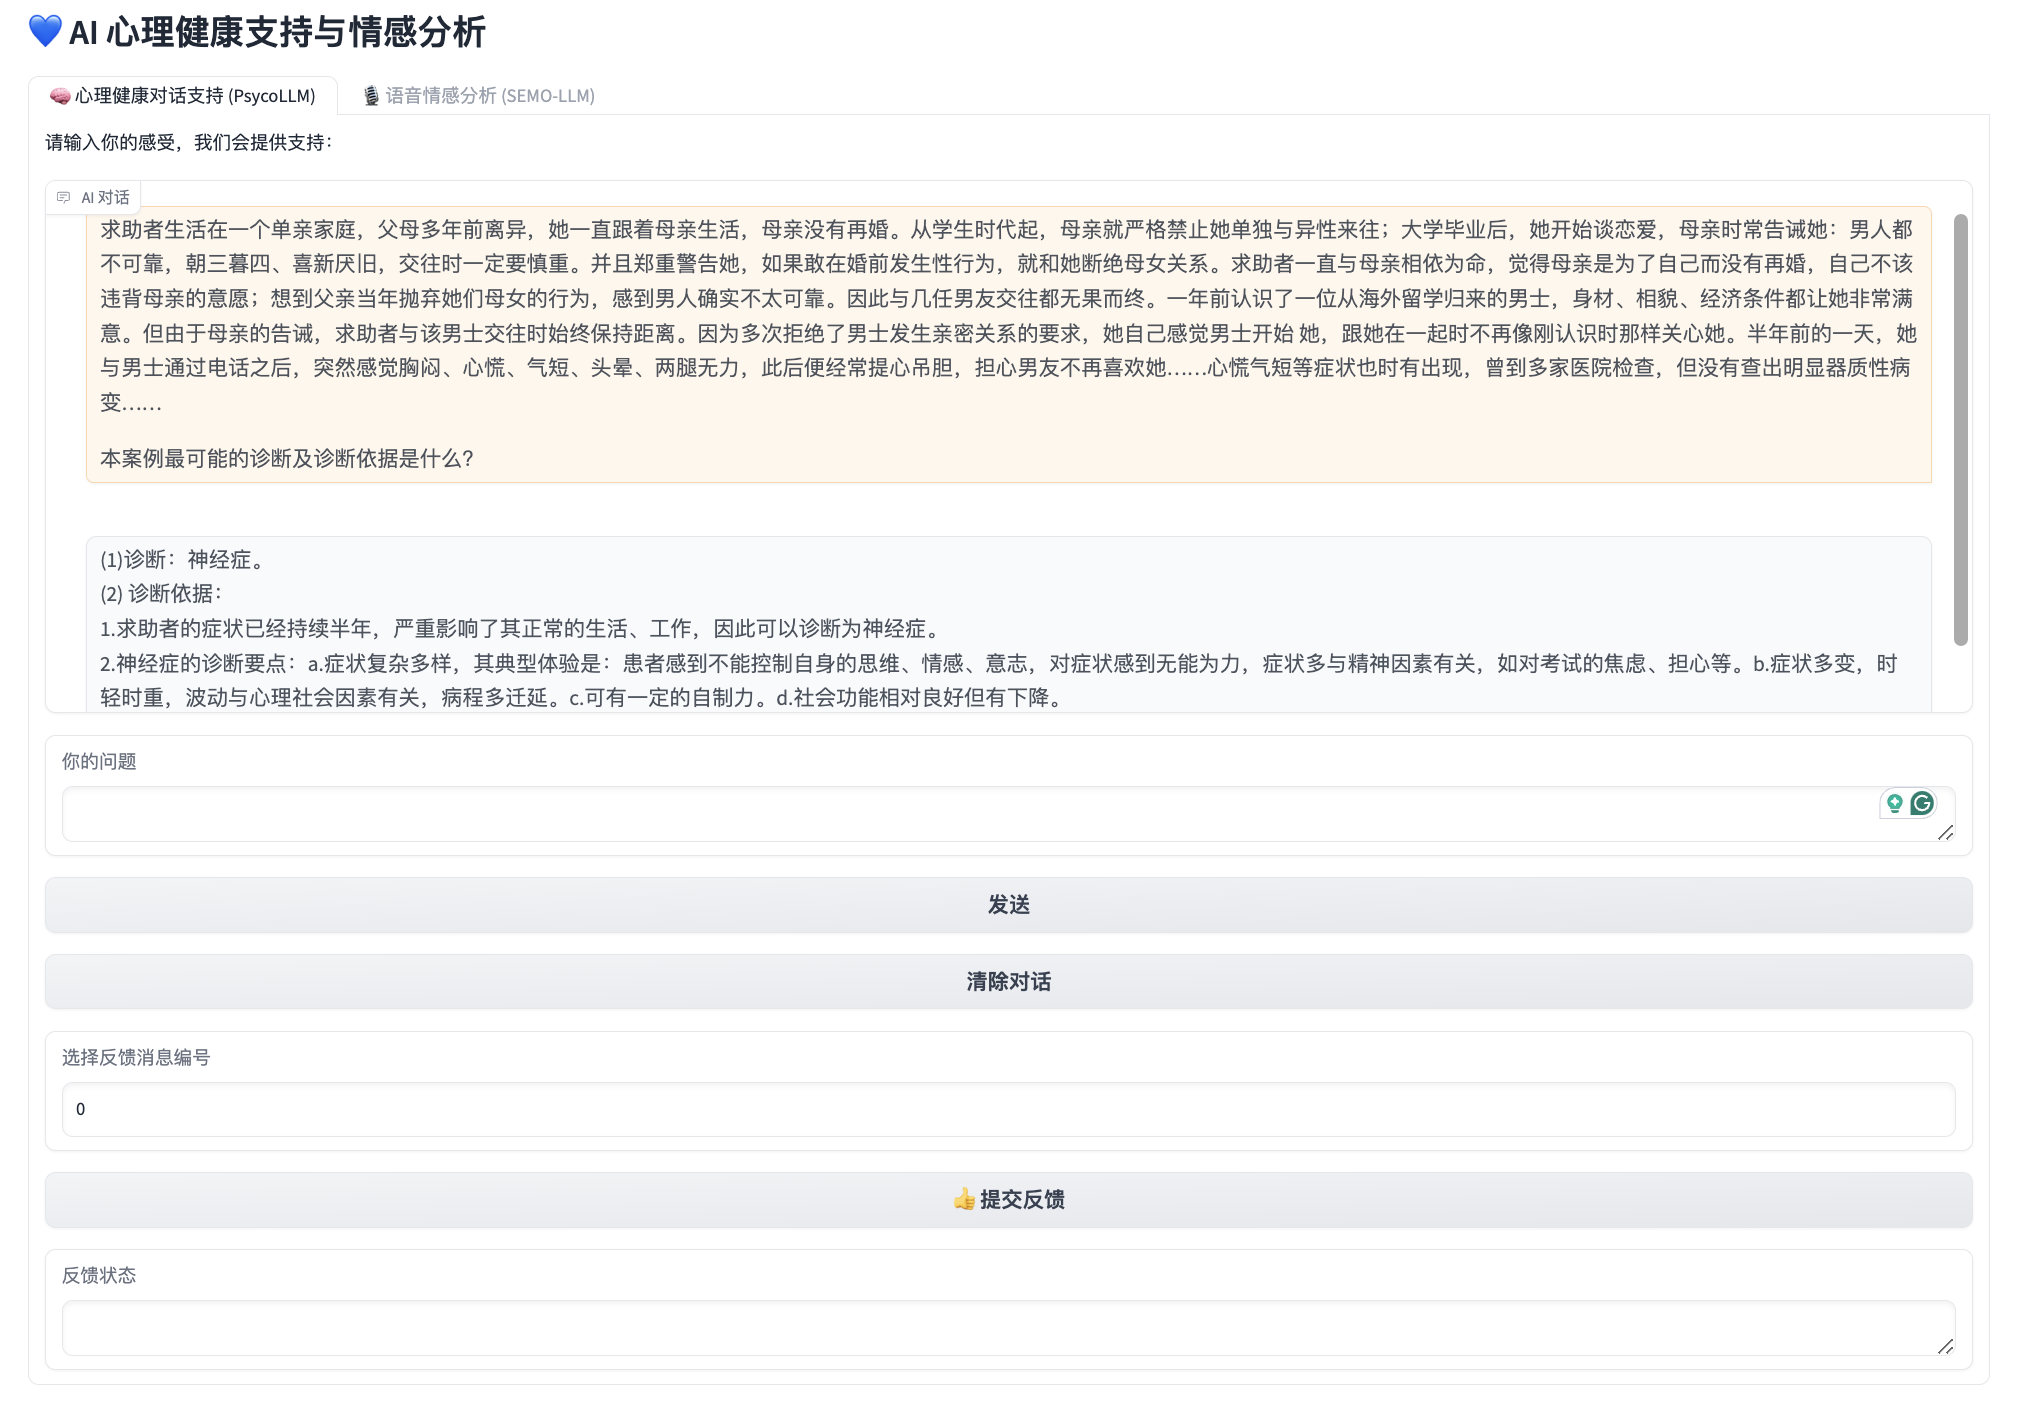
\includegraphics[width=0.8\textwidth]{demo4.png}
  \caption{心理健康诊断结果展示}
  \label{fig:心理健康诊断结果展示}
\end{figure}

\begin{figure}[ht]
  \centering
  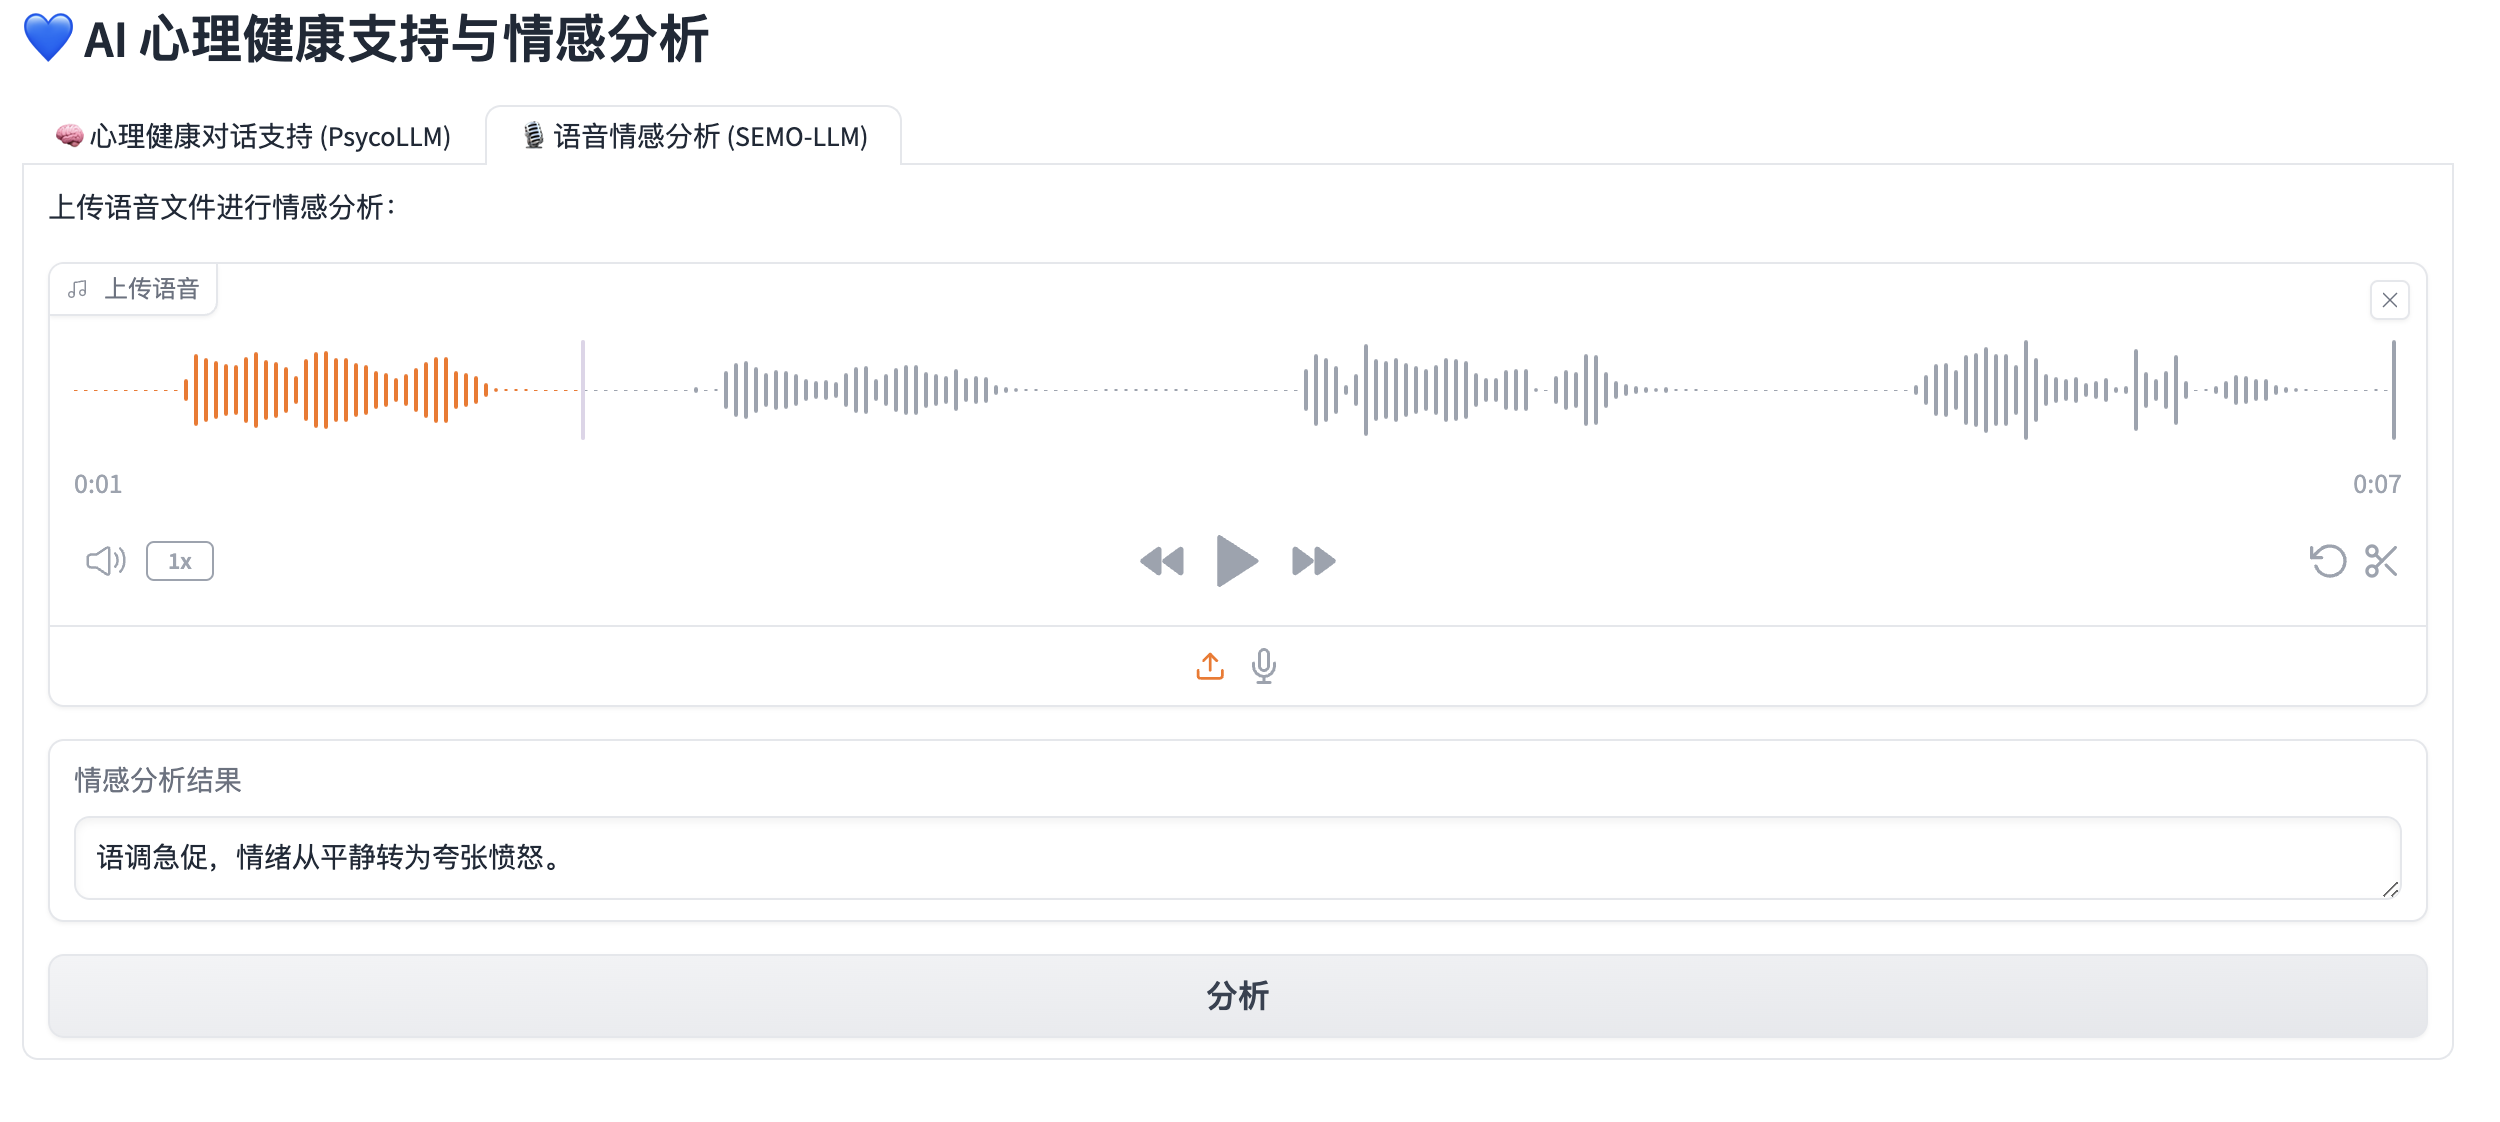
\includegraphics[width=1\textwidth]{demo5.png}
  \caption{语音情感描述结果展示}
  \label{fig:语音情感描述结果展示}
\end{figure}

\section{软件使用流程}

本系统的使用流程涵盖从用户数据输入、模型推理、结果展示到个性化反馈的完整闭环,旨在提供高效、精准的心理健康咨询和情感分析服务。用户可以通过文本输入或语音输入两种方式与系统交互,系统依托心理大模型(PsycoLLM)和多模态情感描述模型(SEMO-LLM),为用户提供专业的心理咨询问答和情感分析建议,最终通过可视化模块呈现输出结果。

当用户首次访问系统时,将进入主界面,其中提供“心理健康对话支持”和“语音情感分析”两大核心功能。用户可根据需求选择相应的分析模式,心理咨询情感对话功能主要针对文本输入,允许用户输入心理健康相关问题,并获取基于专业心理学知识的问答支持;而语音情绪分析功能支持用户上传语音数据,系统将解析语音情绪状态,并生成相应的情感描述。在用户选择功能后,进入数据输入阶段,用户可以通过文本框输入心理咨询问题,或通过麦克风录音/上传音频文件进行语音数据输入。文本输入将在后台经过敏感词过滤、去除空白符等预处理,而语音输入则通过WavLM-Large 模型提取音频特征,包括语速、音调、情感倾向等,并转换为文本以进一步处理。

数据输入完成后,系统进入模型推理阶段,根据用户选择的功能调用不同的模型进行推理。当用户选择心理咨询情感对话时,系统会调用 PsycoLLM,提供基于专业心理学理论的回答,确保输出内容的科学性和合理性。系统还具备多轮对话能力,能够基于用户的连续输入,进行上下文语境理解,使得对话更加自然流畅。当用户选择语音情感描述分析时,系统会调用 SEMO-LLM,先对语音进行特征对齐,利用稀疏桥接 Transformer 将音频特征转换为与文本兼容的情感特征,并结合情感描述 Prompt 进行文本生成,输出对应的情感描述,如“语调急促,情绪从平静转为夸张愤怒。”。

模型推理完成后,系统进入结果展示与交互阶段。所有心理咨询回答和情感描述都会通过可视化模块进行展示,包括流式文本输出、用户情绪状态趋势图等。例如,对于心理咨询结果,系统会提供关键词云图,帮助用户理解核心建议;用户还可以对模型回答进行评分,提供用户反馈,以便系统优化后续的咨询质量。此外,系统还提供历史交互记录,用户可随时查看过往的心理咨询对话,或分析自己一段时间内的情绪变化趋势。

当用户完成咨询或情感分析后,可以选择结束使用或重新开始。整个软件使用流程确保用户能够获得智能化、精准、高效、安全的心理健康对话支持和语音情感描述分析服务。

\section{本章小结}

% 本章围绕大模型心理与情绪分析系统的软件设计与实现进行了详细阐述,主要涵盖系统分析与总体设计、系统功能模块设计以及软件使用流程三个方面。(1)首先,在系统分析与总体设计部分,明确了系统的功能需求,包括支持文本和语音两种输入模态,提供智能心理问答、语音情感描述、心理评估与反馈,以及可视化展示等核心功能。系统基于心理大模型 PsycoLLM 和多模态情感描述模型 SEMO-LLM,利用大规模心理学知识训练大语言模型,并结合多轮对话理解和语音情绪分析技术,以实现更加自然的心理咨询对话和精准的情绪解析。(2)随后,介绍了系统功能模块设计,系统由四个核心功能模块组成:数据输入模块、智能心理问答模块、语音情感描述模块和可视化展示模块。数据输入模块支持用户通过文本框或语音输入进行交互,并采用文本预处理和语音特征提取技术,确保数据的质量和可用性;智能心理问答模块基于 PsycoLLM,提供高质量的心理咨询问答和多轮情感交互,确保生成回答的专业性和连贯性;语音情感描述模块基于 SEMO-LLM,通过 WavLM-Large 提取语音特征,并结合稀疏桥接 Transformer 进行特征对齐,以生成符合用户情绪状态的情感描述信息;可视化展示模块通过流式解码方式,使用户能够直观理解系统输出的心理健康分析结果。(3)最后,在软件使用流程部分,详细介绍了系统的操作步骤,从用户进入系统、选择功能、输入数据、模型推理、结果展示到个性化推荐等各个环节进行了完整描述,确保用户能够流畅地使用系统并获得精准的心理健康对话支持。
本章围绕大模型心理与情绪分析系统的软件设计与实现进行了详细阐述,主要涵盖系统分析与总体设计、系统功能模块设计及软件使用流程三个方面。(1)系统分析与总体设计:首先,明确了系统的功能需求,包括支持文本与语音两种输入模态,并提供智能心理问答、语音情感描述、心理评估与反馈以及可视化展示等核心功能。系统基于心理大模型 PsycoLLM 和 多模态情感描述模型 SEMO-LLM,通过大规模心理学知识训练的语言模型,结合多轮对话理解与语音情绪分析技术,实现更自然的心理咨询交互和更精准的情绪解析。(2)系统功能模块设计:系统由四个核心模块组成,即数据输入模块、智能心理问答模块、语音情感描述模块和可视化展示模块。数据输入模块 支持用户通过文本框或语音输入进行交互,并通过文本预处理和语音特征提取技术,确保数据的质量与可用性;智能心理问答模块 基于 PsycoLLM,提供高质量的心理咨询问答和多轮情感交互,以确保生成内容的专业性与连贯性;语音情感描述模块 依托 SEMO-LLM,结合 WavLM-Large 进行语音特征提取,并利用稀疏桥接 Transformer 进行特征对齐,以生成符合用户情绪状态的情感描述文本;可视化展示模块 采用流式解码方式,使用户能够直观理解系统输出的心理健康分析结果。(3)软件使用流程:最后,详细介绍了系统的操作流程,包括用户进入系统、选择功能、输入数据、模型推理、结果展示以及个性化推荐等环节,确保用户能够顺畅使用系统,并获得精准的心理健康支持。

